\documentclass[11pt]{article}
\usepackage{geometry}                % See geometry.pdf to learn the layout options. There are lots.
\geometry{letterpaper}                   % ... or a4paper or a5paper or ... 
%\geometry{landscape}                % Activate for for rotated page geometry
%\usepackage[parfill]{parskip}    % Activate to begin paragraphs with an empty line rather than an indent
\usepackage{graphicx}
\usepackage{amssymb,amsmath}
\usepackage{epstopdf}
\usepackage{pgf}
\usepackage{pgfpages}
\usepackage{tikz}
\usetikzlibrary{arrows,backgrounds}
\usepgflibrary{shapes}
\DeclareGraphicsRule{.tif}{png}{.png}{`convert #1 `dirname #1`/`basename #1 .tif`.png}
\pagestyle{empty}


\begin{document}

   \begin{center}
     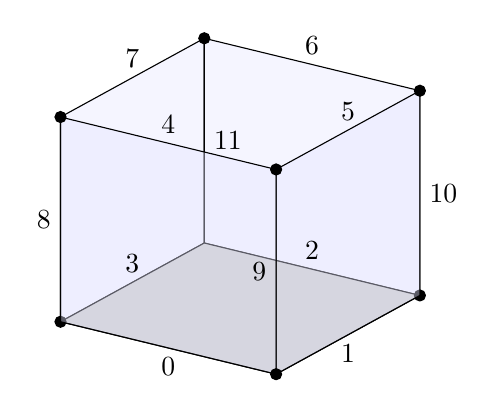
\begin{tikzpicture}[join=round] % Hexahedron Edges
         \filldraw[fill=blue!10,fill opacity=0.4](-2.282,2.433)--(-2.282,-.167)--(-.456,.833)--(-.456,3.433)--cycle;
         \filldraw[fill=blue!10,fill opacity=0.4](-.456,3.433)--(-.456,.833)--(2.282,.167)--(2.282,2.767)--cycle;
         \filldraw[fill=black!20](2.282,.167)--(-.456,.833)--(-2.282,-.167)--(.456,-.833)--cycle;
        \filldraw(-.456,3.433) circle (2pt);
        \filldraw(2.282,.167) circle (2pt);
         \filldraw[fill=blue!10,fill opacity=0.4](2.282,2.767)--(2.282,.167)--(.456,-.833)--(.456,1.767)--cycle;
        \filldraw(-2.282,-.167) circle (2pt);
         \filldraw[fill=blue!10,fill opacity=0.4](.456,1.767)--(.456,-.833)--(-2.282,-.167)--(-2.282,2.433)--cycle;
        \filldraw(2.282,2.767) circle (2pt);
        \filldraw(-2.282,2.433) circle (2pt);
        \filldraw(.456,-.833) circle (2pt);
        \filldraw(.456,1.767) circle (2pt);
         \fill[black]
                (-.913,-.5) node [below] {0}
                (1.369,-.333) node [below] {1}
                (.913,.5) node [above] {2}
                (-1.369,.333) node [above] {3}
                (-2.282,1.133) node [left] {8}
                (.456,.467) node [left] {9}
                (2.282,1.467) node [right] {10}
                (-.456,2.133) node [right] {11}
                (-.913,2.1) node [above] {4}
                (1.369,2.267) node [above] {5}
                (.913,3.1) node [above] {6}
                (-1.369,2.933) node [above] {7};
     \end{tikzpicture}
  \end{center}
\end{document}  
